\documentclass[11pt, oneside]{article}   	% use "amsart" instead of "article" for AMSLaTeX format
\usepackage{geometry}                		% See geometry.pdf to learn the layout options. There are lots.
\geometry{letterpaper}                   		% ... or a4paper or a5paper or ... 
%\geometry{landscape}                		% Activate for for rotated page geometry
%\usepackage[parfill]{parskip}    		% Activate to begin paragraphs with an empty line rather than an indent
\usepackage{graphicx}				% Use pdf, png, jpg, or eps� with pdflatex; use eps in DVI mode
								% TeX will automatically convert eps --> pdf in pdflatex		
\usepackage{amssymb}
\usepackage{amsmath}
\usepackage{parskip}


\title{Limits-Problems}
%\author{The Author}
%\section{}
% \subsection*{R code}
\date{}							% Activate to display a given date or no date

\graphicspath{{/Users/telliott_admin/Dropbox/Tex/png/}}
% \begin{center} 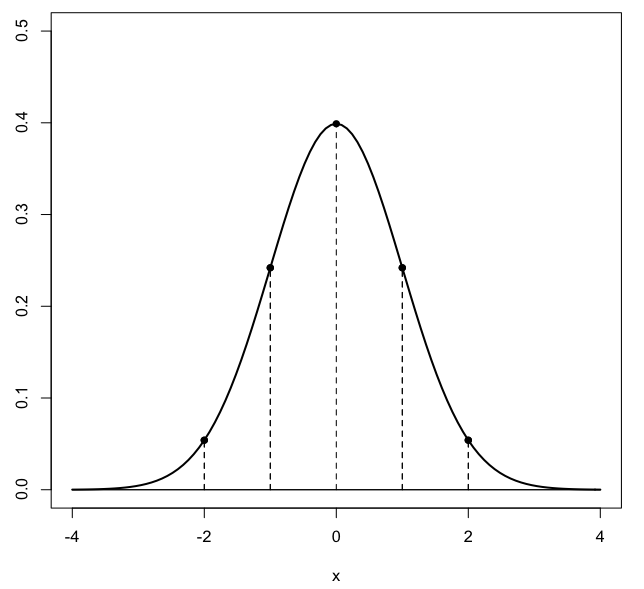
\includegraphics [scale=0.4] {gauss3.png} \end{center}

\begin{document}
\maketitle
\large

The \emph{Calculus Lifesaver} has a very nice treatment of limits, both theoretically and practically.  The first thing is to note that the techniques differ depending on whether the limit is at a number $a$ which $x$ approaches, $x \rightarrow a$, or as $x$ approaches infinity, either plus or minus.  Start with the first type, $x \rightarrow a$.

Try plugging in $x=a$ and see what happens.  (Maybe there is no problem).

Next, for rational functions such as

\[ \lim_{x \rightarrow a} \ \frac{p(x)}{q(x)} \]

try factoring.  (Since we are interested in the limit, and not directly in what happens when $x$ is equal to $a$, if we can get a term $(x-a)$ in both the numerator and denominator, it will lead to simplification).

\subsection*{Factoring}

Factoring is OK when evaluating a limit.  For example

\[ \lim_{x \rightarrow 2} \ \frac{x^2 + 4x - 12}{\ x^2-2x} \]

Plugging in $x=2$ gives $0/0$.  We notice that we can factor the numerator and the denominator

\[ = \lim_{x \rightarrow 2} \ \frac{(x+6)(x-2)}{\ x(x-2)} \]

Now, since we are \emph{not interested} in what happens at $x=2$, we can cancel here, giving

\[ = \lim_{x \rightarrow 2} \ \frac{(x+6)}{x} = \frac{8}{2} = 4 \]

A harder example might be cubic or higher.

\[ \lim_{x \rightarrow 3} \ \frac{x^3 - 27}{x^4 - 5x^3 + 6x^2}  \]

Recall that 

\[ a^3 - b^3 = (a-b)(a^2 + ab + b^2) \]

Hence we have

\[ \lim_{x \rightarrow 3} \ \frac{(x-3)(x^2 + 3x + 9)}{x^2(x^2 - 5x + 6)}  \]
\[ = \lim_{x \rightarrow 3} \ \frac{(x-3)(x^2 + 3x + 9)}{x^2(x-3)(x-2)}  \]
\[ = \lim_{x \rightarrow 3} \ \frac{x^2 + 3x + 9}{x^2(x-2)}  = \frac{9 + 9 + 9}{9} = 3 \]

If, when we plug in $x=a$, only the denominator but not the numerator is zero, then we have one of the following situations:

\begin{center} 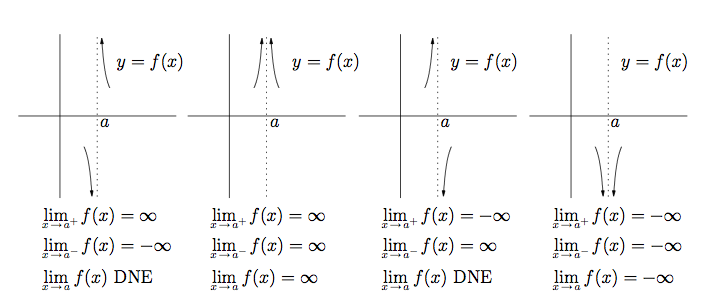
\includegraphics [scale=0.5] {limits1.png} \end{center}

An example:

\[ \lim_{x \rightarrow 1} \ \frac{2x^2 -x - 6}{x(x-1)^3}  \]

At $x=1$, the numerator is equal to $-5$, and will not change sign if x is slightly smaller or larger than $1$.  Similarly for $x$ in the denominator.  However, $x-1$ does change sign, and so does $(x-1)^3$.

We have the situation shown in the left-hand panel above, and since the two limits $x \rightarrow a+$ and $x \rightarrow a-$ are not equal, the limit $x \rightarrow a$ does not exist (DNE).

On the other hand, if we have the similar but slightly changed

\[ \lim_{x \rightarrow 1} \ \frac{2x^2 -x - 6}{x(x-1)^2}  \]

Now the denominator does not change sign and is positive, hence both the one-sided limits are equal to $-\infty$, and so the limit is also equal to $-\infty$.

For limits involving square roots, we use the conjugate.

\subsection*{Conjugate}
\[ \lim_{x \rightarrow 4} \ \frac{\sqrt{x} - 2}{\ x-4} \]

Substitution gives $0/0$.  

The conjugate of $\sqrt{x} - 2$ is $\sqrt{x} + 2$.  The point is that the product does not contain a square root:

\[ (\sqrt{x} - 2) \times (\sqrt{x} + 2) = x - 4 \]


We try multiplication by the conjugate

\[ \frac{\sqrt{x} - 2}{\ x-4} = \frac{\sqrt{x} - 2}{\ x-4} \ \frac{\sqrt{x} + 2}{\sqrt{x} + 2} \]

The numerator gives $x-4$, and  before you rush to do the denominator, notice the cancellation:
\[ = \frac{x - 4}{(x-4)(\sqrt{x} + 2)} \]
So this is just
\[ \lim_{x \rightarrow 4} \  \frac{1}{\sqrt{x} + 2} = \frac{1}{4}  \]

A slightly more complicated example:

\[  \lim_{x \rightarrow 5} \  \frac{\sqrt{x^2 -9} - 4}{x-5}   \]
\[  = \lim_{x \rightarrow 5} \  \frac{\sqrt{x^2 -9} - 4}{x-5} \times   \frac{\sqrt{x^2 -9} + 4}{\sqrt{x^2 -9} + 4}  \]
\[  = \lim_{x \rightarrow 5} \  \frac{x^2 - 9 - 16}{(x-5)(\sqrt{x^2 -9} + 4)}  \]

The numerator becomes $x^2 - 25 = (x-5)(x+5)$ leading to a cancellation.  The result is

\[  = \lim_{x \rightarrow 5} \  \frac{x+5}{\sqrt{x^2 -9} + 4} = \frac{10}{4+4}  \]

Now we deal with $\infty$.

\subsection*{Polynomial as $x \rightarrow \infty$}
\[ \lim_{x \rightarrow \infty} \ 3x^2 + 2x + 1 \]
\[ = \lim_{x \rightarrow \infty} \ x^2 (3 + \frac{2}{x} + \frac{1}{x^2}) \]
\[ = \lim_{x \rightarrow \infty} \ x^2 (3 + 0 + 0 ) \]
\[ = \lim_{x \rightarrow \infty} \ 3x^2  =  \infty \]

This method can be adapted to more complex examples.

\[ = \lim_{x \rightarrow \infty} \ \frac{2x^4 - x^2 + 8x}{-5x^4 + 7}  \]
\[ = \lim_{x \rightarrow \infty} \ \frac{(2 - \frac{1}{x^2} + \frac{8}{x^3})(x^4)}{(-5 + \frac{7}{x^4})(x^4)}  \]
\[ = \lim_{x \rightarrow \infty} \ \frac{(2 - 0 + 0)(x^4)}{(-5 + 0)(x^4)} = - \frac{2}{5}  \]

And one with a square root

\[ \lim_{x \rightarrow \infty} \ \frac{\sqrt{3x^2 + 6}}{5 - 2x}  \]
\[ = \lim_{x \rightarrow \infty} \ \frac{\sqrt{x^2} \sqrt{3 + \frac{6}{x^2}}}{x(\frac{5}{x} - 2)}  \]
\[ = \lim_{x \rightarrow \infty} \ \frac{\sqrt{x^2} \sqrt{3 + 0}}{x(0 - 2)}  \]

But we have to be careful here because
\[ \sqrt{x^2} = | x | \]  
So this is 
\[ = -\frac{\sqrt{3}}{2} \  \lim_{x \rightarrow \infty} \ \frac{| x |}{x} \]

which we deal with now.

\subsection*{absolute value}

Consider

\[ \lim_{x \rightarrow 0} \ \frac{|x|}{x}  \]

At $x=0$ , this is equal to $0/0$.  Also, for any $x \ne 0$

\[ \lvert \frac{|x|}{x} \rvert = 1 \]

Now, what happens as we approach $x=0$ from either side?  Approaching from the right, for $x > 0$, the sign of the expression is positive, while approaching from the left, for $x < 0$, the sign is negative.  Thus, the limit as $x \rightarrow 0-$ is not equal to the limit as 
$x \rightarrow 0+$ and so the two-sided limit as $x \rightarrow 0$ does not exist.

For the problem we had above

\[ \lim_{x \rightarrow \infty} \ \frac{| x |}{x} \]

Since as $x \rightarrow \infty$,  $x>0$, since both terms of the fraction are positive, the limit is $+1$.

This problem is only slightly different:

\[ \lim_{x \rightarrow -2} \ \frac{|x+2|}{x+2}  \]

Again, for every $x  \ne -2$, the absolute value of the expression is equal to $1$, but the sign changes depending from which side we are approaching to the limit.  From the left, the value is -1 because the sign of the denominator is less than zero.  Hence, the two-sided limit does not exist.

\subsection*{Sine}

As you know, $\sin x$ does not approach any limit because it is periodic.  So what about 
\[ \lim_{x \rightarrow 0} \ x \sin x \]
We may guess that since the right-hand term is always a number between $-1$ and $1$, when multiplied by $0$ we'll get $0$.  The way to do this is to use the "squeeze" theorem.

\[ -1 \le \sin x \le 1 \]
When we multiply by $x$, we have to take account of sign.  So let's do the two cases separately.  For $x > 0$, we obtain
\[ -x \le x \sin x \le x \]
Since both $-x$ and $x$ go to $0$, so does $x \sin x$.  Suppose $x < 0$.  Then, when we multiply we have to flip the inequality
\[ -x \ge x \sin x \ge x \]
but it doesn't matter because both left and right-hand terms still tend to $0$, and since $x \sin x$ is squeezed between them, it does too.

\end{document}  